\chapter{Experiments and Results}
\label{cha:experiments}

As multiple approaches were developed during the thesis, several experiments were required. These experiments can be categorized into 

\begin{itemize}
\item memory usage
\item file size
\item time required to
    \begin{itemize}
    \item load the database
    \item extract codebooks from the database
    \item do a complete query run
    \end{itemize}
\item detection performance
\end{itemize}

To test the loading times, the different storage mechanisms were each tested with 512 and 1000 codebook dimensions. Together with the different mechanism, this results in total to 14 unique combinations. Each combination loads the same database containing 50 images with an average size of 476x391 pixels\footnote{The list of PASCAL ids can be found in the appendix \ref{apx:images50}}. It should be noted that all mechanisms result in the same integral images at runtime or at least provide the same results on extraction.

\begin{figure}
\centering
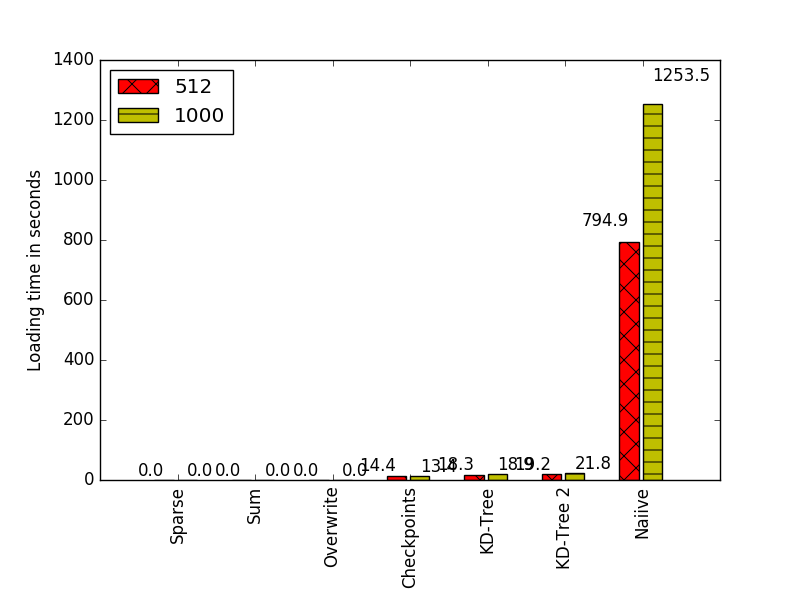
\includegraphics[width=0.7\linewidth]{images/loading_time}
\caption{Loading times of all database storage backends.}
\label{fig:loading_all}
\end{figure}


\begin{figure}
\centering
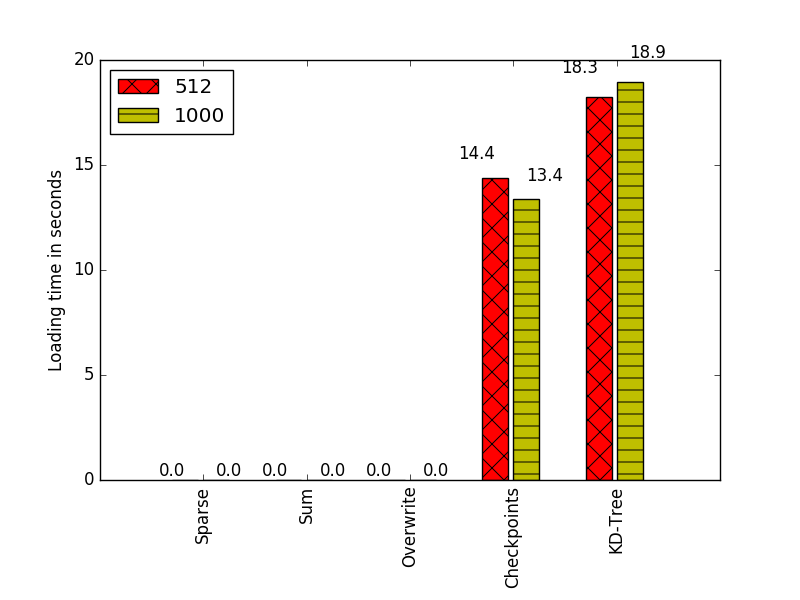
\includegraphics[width=0.7\linewidth]{images/loading_time_2}
\caption{Loading times of all database storage backends except the na\"{\i}ve and sparse ones.}
\label{fig:loading_except_naiive}
\end{figure}


As one can see in \figref{loading_all} the na\"{\i}ve approach (which stores the complete matrices) obviously requires an unusable amount of time to load the database. One reason that the loading time does not have a linear dependency on the codebook size, is that \MATLAB uses a compression for files with version 7 and above and the possibility for empty codebook entries or similar entries increases for higher dimensional vectors. The approach which stores only a sparse representation with zero values removed, was much faster, but still requires to much time to load compared to the whole computing time of the ExemplarSVM algorithm (85 seconds for 50 images). In \figref{loading_except_naiive} one can see the loading times without the na\"{\i}ve and sparse approaches as they are too close to each other compared to these two approaches.


\begin{figure}
\centering
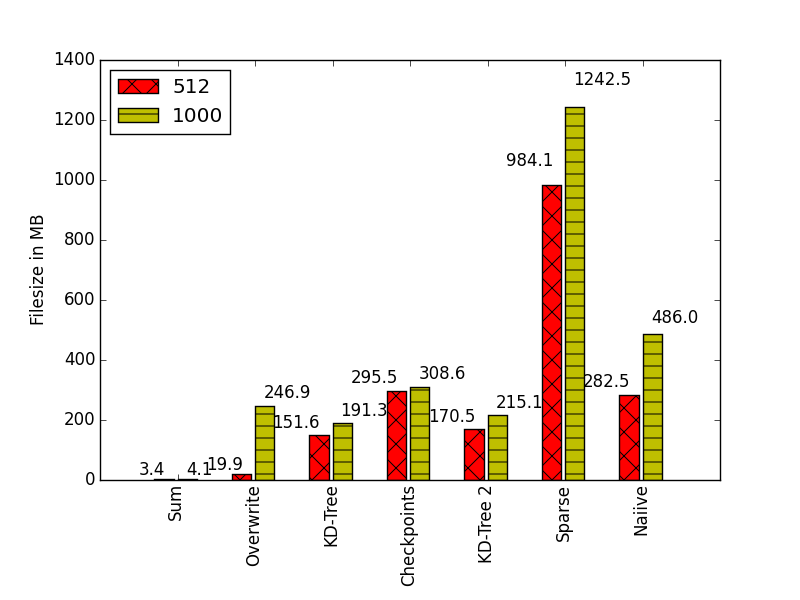
\includegraphics[width=0.7\linewidth]{images/file_size}
\caption[File sizes of the different storage backends]{File sizes of the different storage backends. These are mostly based on the compression of the data and have the most impact on network file storages.}
\label{fig:file_sizes}
\end{figure}

\Figref{file_sizes} shows the file sizes of the different techniques. As one may notice, the \MATLAB sparse representation of the database requires much more space on the filesystem compared to the na\"{\i}ve approach, but loads faster. This is because the internal representation of the sparse matrices was not as small compressed as the full matrices, possibly mainly because the amount of consecutive data is much reduced. Obviously, the compressed matrices have to be uncompressed during load, which requires more time than loading the bigger file of sparse matrices. As the compression is mandatory for \MATLAB files with version 7 and up\footnote{\label{footnote:matlab_files}As described on \url{https://de.mathworks.com/help/matlab/ref/save.html?refresh=true} (visited 11/06/2015)} and version 7.3 is required due to the large variable sizes\footnoteref{footnote:matlab_files}, this behavior can not be circumvented.


\begin{figure}
\centering
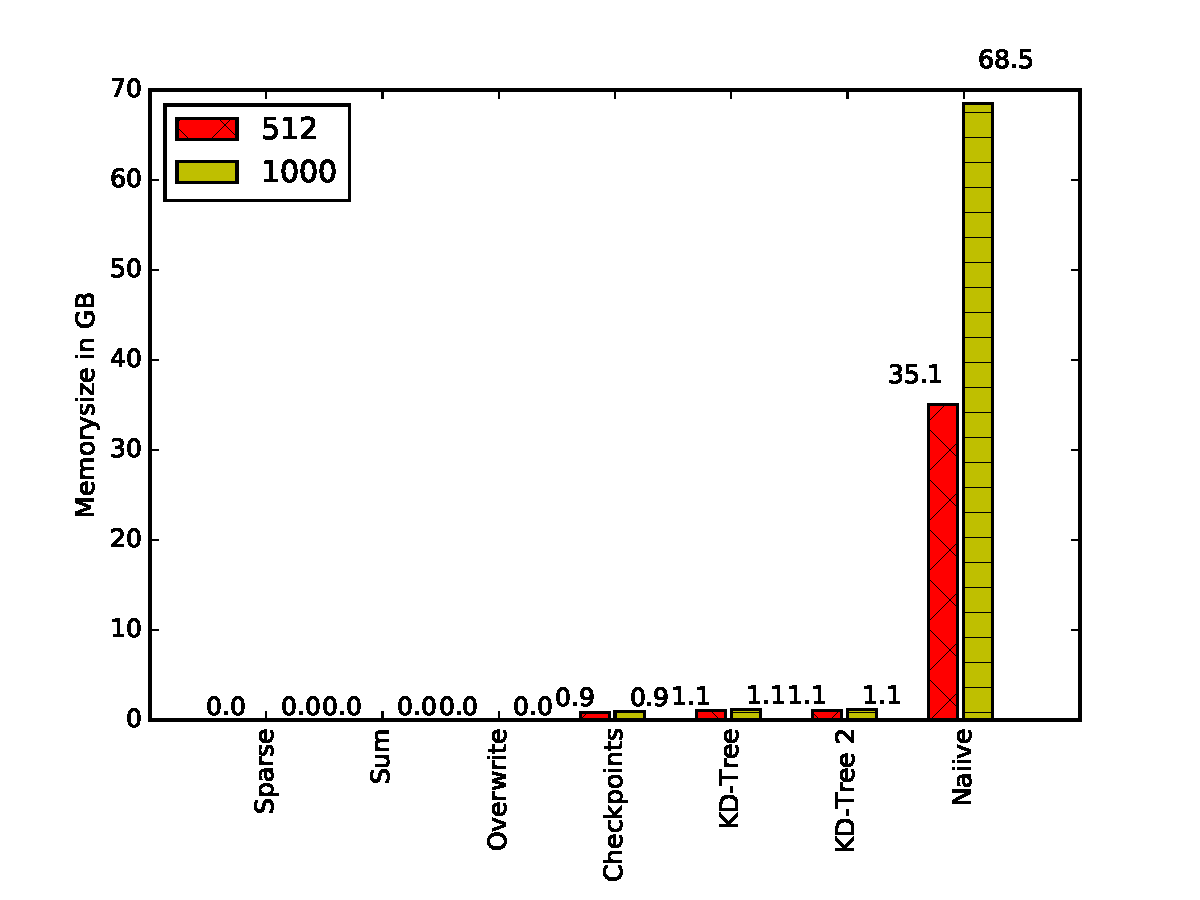
\includegraphics[width=0.7\linewidth]{images/mem_size}
\caption{Memory usage of the different storage backends.}
\label{fig:memory_usage}
\end{figure}

The memory usage of the different techniques in \ac{RAM} is shown in \figref{memory_usage}. It has to be noted that some of the techniques (namely the summation and overwrite) require the reconstruction of the original integral images. This increases the memory usage during runtime, but (in contrast to the na\"{\i}ve technique) only for one image at a time (when it is queried). The required size depends on the information which is needed to reconstruct every possible extraction point. As the summation techniques calculates the integral image at runtime, it requires the least stored information. The implementation of the sparse storage mechanism allows only to omit cells with a zero value and therefore has to store all cells which are in the bottom left of the first filled cell for a codebook dimension. The kd-Tree variants, compared to the checkpoints variant, require some additional meta information to build up the tree.

To complete the comparison between the different mechanisms, the time required to extract a complete set of windows from an image was measured. The computation of the window list was based on \textit{2008\_004363.jpg} with the bounding box $x_{min} = 102, y_{min} = 178, x_{max} = 344, y_{max} = 336$. This results into 4784 windows. %TODO: Extract time

As the ExemplarSVM does not load precomputed data, except of the negative features for the \ac{SVM} training, it was not possible to compare it with the different parts of the tested approaches. Instead the total processing time is used.
With the initial implementation, which uses a sliding window algorithm with a fixed 10 pixel shift, the amount of searched windows (between 4000 and 7500, depending on the query image) is much higher compared to the searched windows in the ExemplarSVM algorithm (limited to 400). This obviously results in a high processing time for all configurations as one can see in \figref{orig_window_time}.

\begin{figure}
\centering
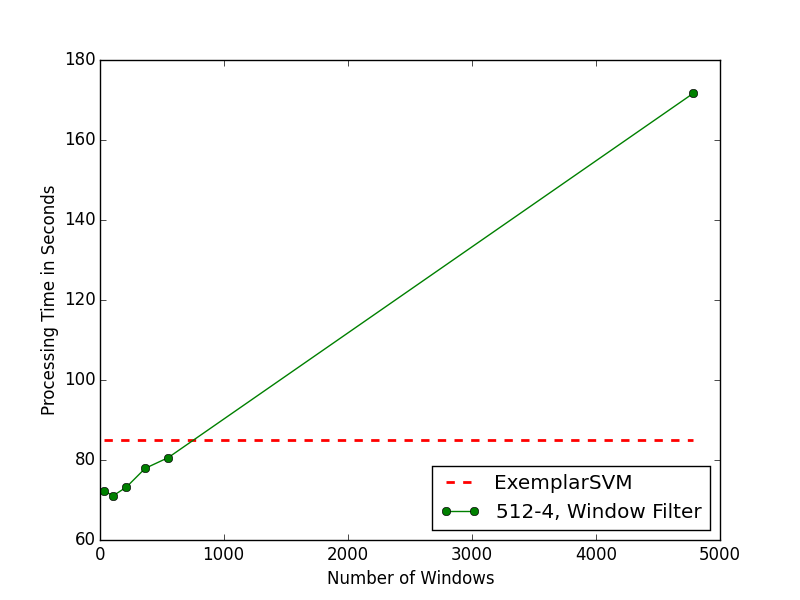
\includegraphics[width=0.7\linewidth]{images/window_comparison-512-4-filtered}
\caption[Window comparison]{Comparison of the processing time of different amount of sliding windows. The red dashed line represents the processing time of an ExemplarSVM search with the same database and query part.}
\label{fig:processing_time_windows}
\end{figure}


Further experiments used an implementation which shifts the windows based on their size. This reduces the amount of windows and therefore increases the processing speed as shown in \figref{processing_time_windows}.
As it obviously also reduces the number of hypotheses, the possibility to find a perfect match decreases. To see the relationship between the amount of windows and the detection performance, multiple runs with different configurations and window slide settings were done.

\begin{figure}
\begin{subfigure}{\textwidth}
\centering
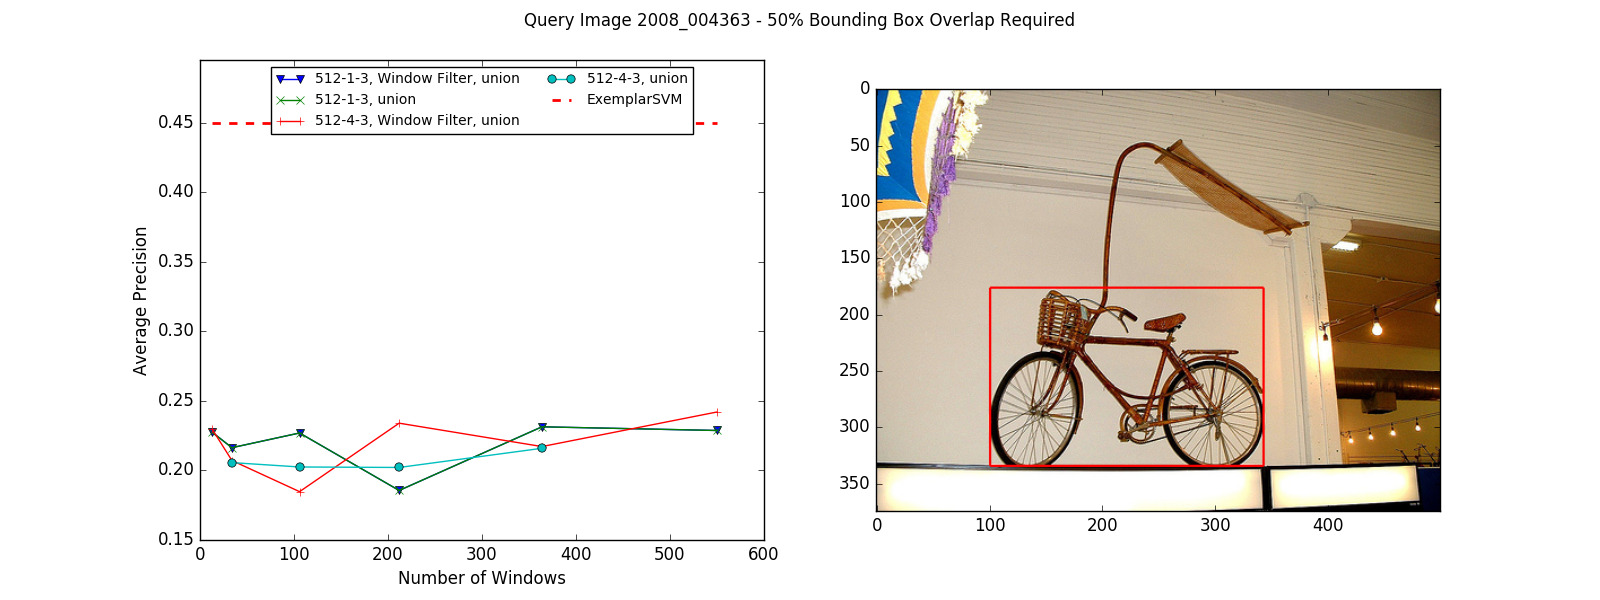
\includegraphics[width=\textwidth]{images/db1_window_comparison-2008_004363}
\end{subfigure}

\begin{subfigure}{\textwidth}
\centering
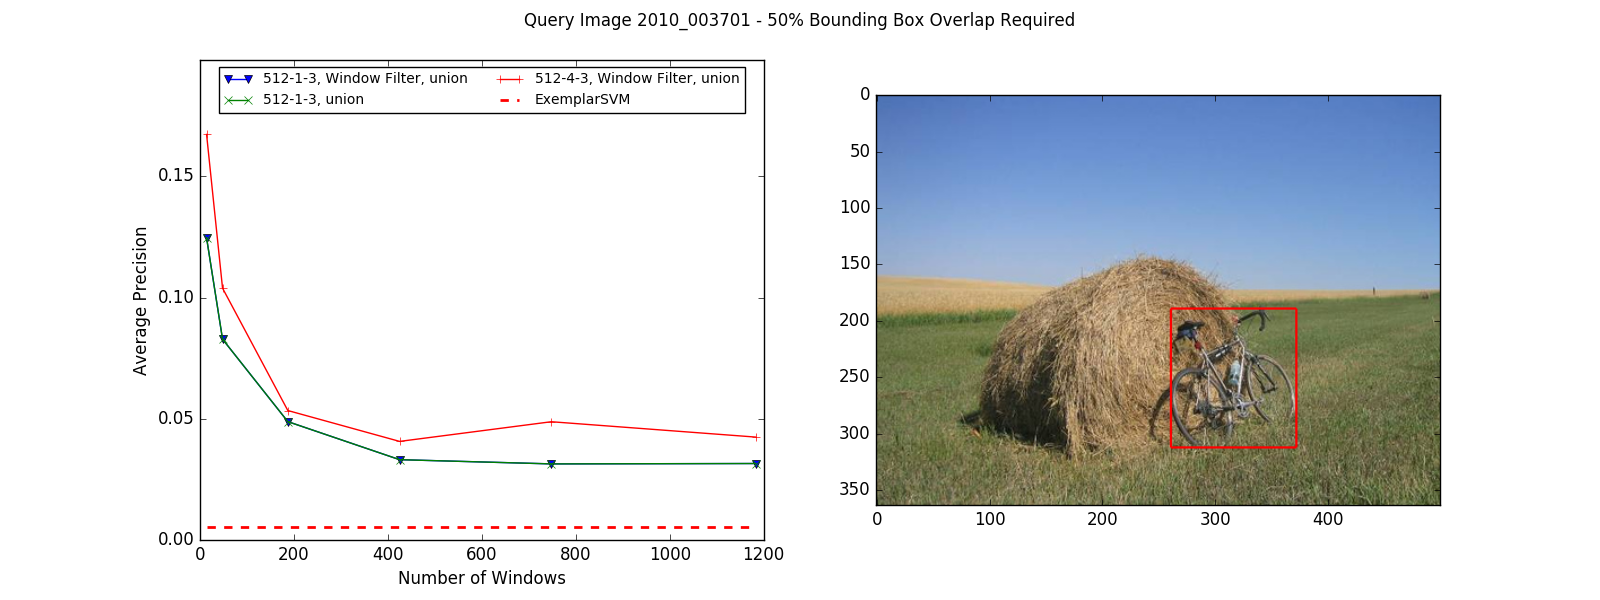
\includegraphics[width=\textwidth]{images/db1_window_comparison-2010_003701}
\end{subfigure}
\caption[Performances of querying with 2008\_004363 and 2010\_003701 with different techniques and window amounts]{Performances of querying with 2008\_004363 and 2010\_003701 with different techniques and window amounts. 512-4-3 represents 512 clusters, windows divided into 4 parts, database splitted into 3 scale ranges.}
\label{fig:performance_query_params}
\end{figure}


The tests with the files from appendix \ref{apx:images50} provided a performance which comes near to the ExemplarSVM. Additionally, some of the query images performed much better compared to the ExemplarSVM algorithm (\figref{performance_query_params}). The significantly performance differences between ExemplarSVM and the tested approaches, together with the fact that the results could not be directly correlated to the chosen parameters, the assumption arises that there is some bias in the test set. This bias results in a behavior which always prefers windows which encloses a large portion of an image. Combined with the fact that (the randomly chosen) test images contain many images with bicycles nearly of the image size, this results in similar performance rates for different bicycle queries. To add more variance to the test set, another randomly chosen images were added to get 234 images in total (97 bicycle and 137 non-bicycle images).

By using this image set, the performance slightly decreased (as expected) (\figref{db2_window_comparison-ALL} compared to \figref{db1_window_comparison-ALL}). Additionally the parameter combination which was expected to provide the best results (4 parts with window prefilter) jumps from the worst to the best. This could be either explained by a measurement error, or because of the increased amount of negatives in the dataset. Therefore result in more penalties if the detection is not accurate enough. The performance compared to the search time is similar to the 50 image dataset, although some of the parameter combinations (primarily 4 parts, single scale range) took more time in average (per processed image in the database) than the ExemplarSVM. This could be explained by the increased general size of the database and the higher amount of data as all different input scales were loaded together.

For the third iteration of the tests, the first 2500 images of the the \ac{VOC2011} bicycle validation dataset were used. This time, the performance gap between the ExemplarSVM and the different approaches increased and the processing time of all parameter combinations was higher than the ExemplarSVM variant. As this also corresponds to the increased loading time of the database (the processing alone was significant lower than the ExemplarSVM in previous experiments), this could be mitigated by loading smaller chunks of the database. This allows to separate the I/O operations from the CPU intensive tasks. Due to the limited time, this adjustment could not be implemented.


\begin{figure}
\centering
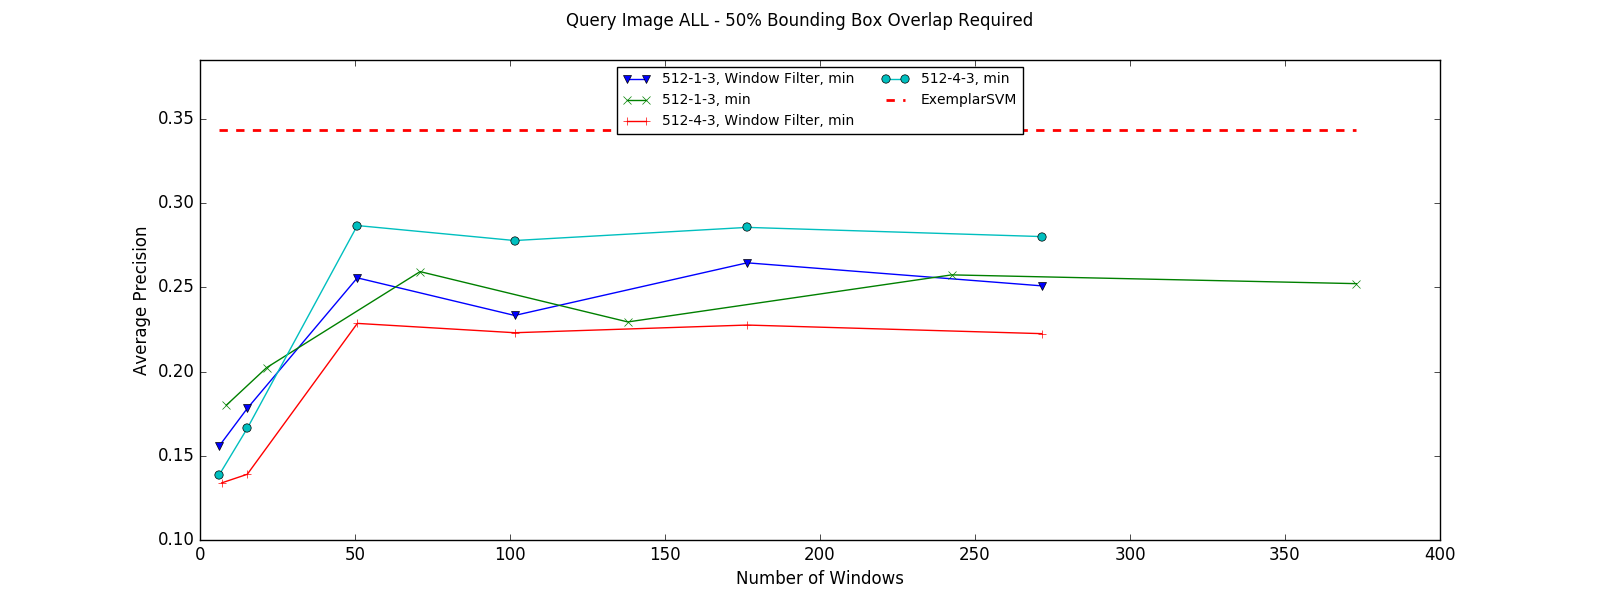
\includegraphics[width=\linewidth]{images/db1_window_comparison-ALL}
\caption{Averaged detection performance of different windows compared to ExemplarSVM (50 images)}
\label{fig:db1_window_comparison-ALL}
\end{figure}


\begin{figure}
\centering
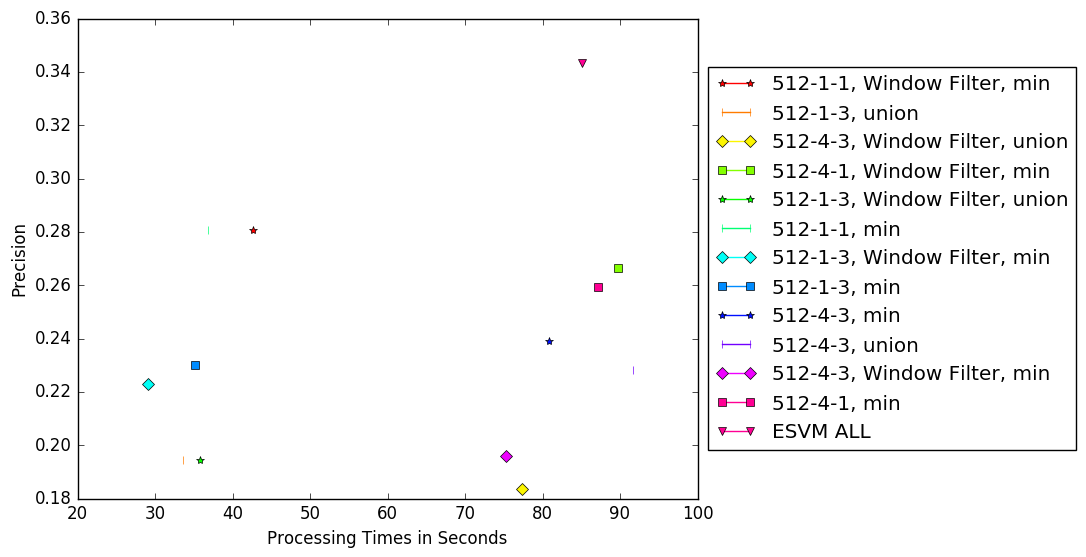
\includegraphics[width=0.7\linewidth]{images/db1_t_vs_p-ALL}
\caption{Performance versus search time (50 images)}
\label{fig:db1_t_vs_p-ALL}
\end{figure}

\begin{figure}
\centering
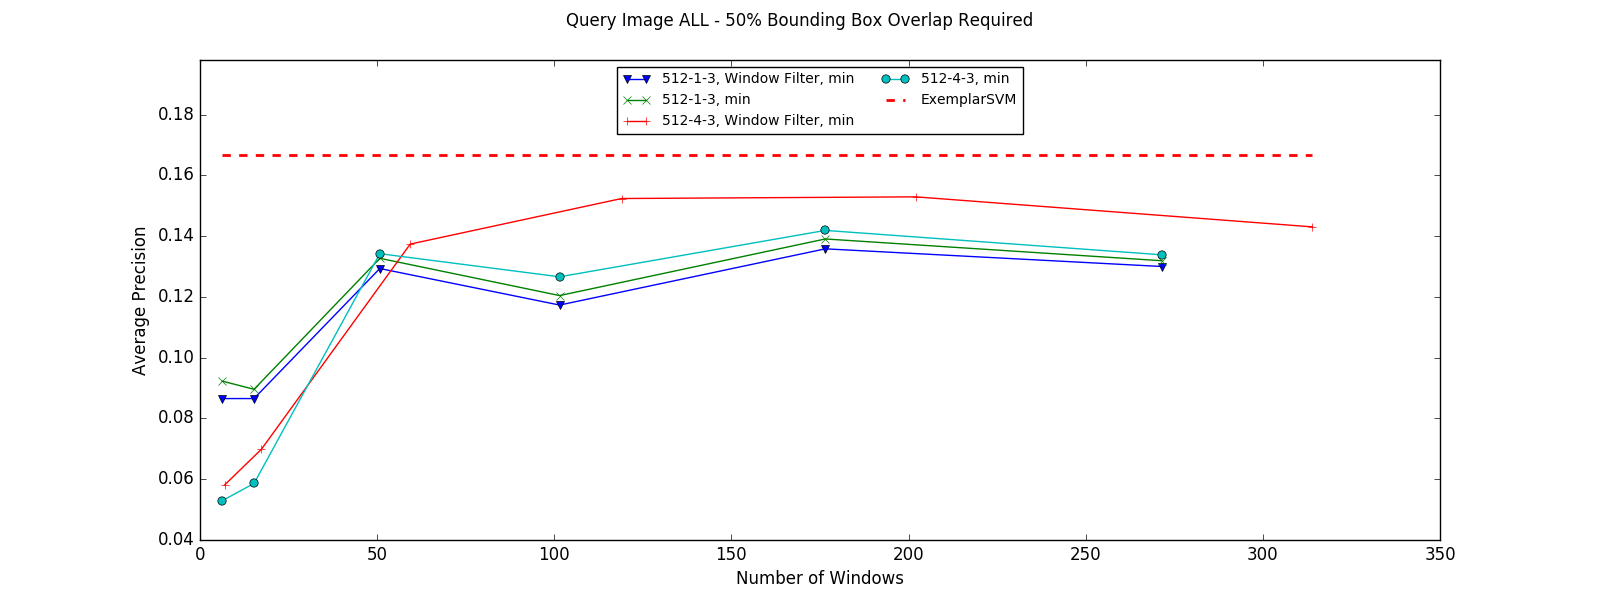
\includegraphics[width=\linewidth]{images/db2_window_comparison-ALL}
\caption{Averaged detection performance of different windows compared to ExemplarSVM (100 images)}
\label{fig:db2_window_comparison-ALL}
\end{figure}


\begin{figure}
\centering
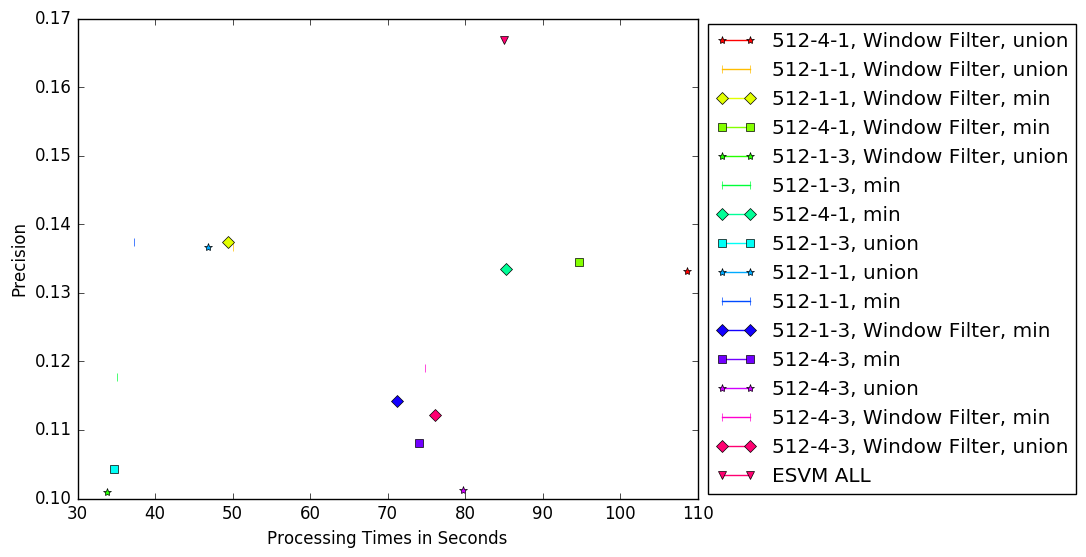
\includegraphics[width=0.7\linewidth]{images/db2_t_vs_p-ALL}
\caption{Performance versus search time (100 images)}
\label{fig:db2_t_vs_p-ALL}
\end{figure}

\begin{figure}
\centering
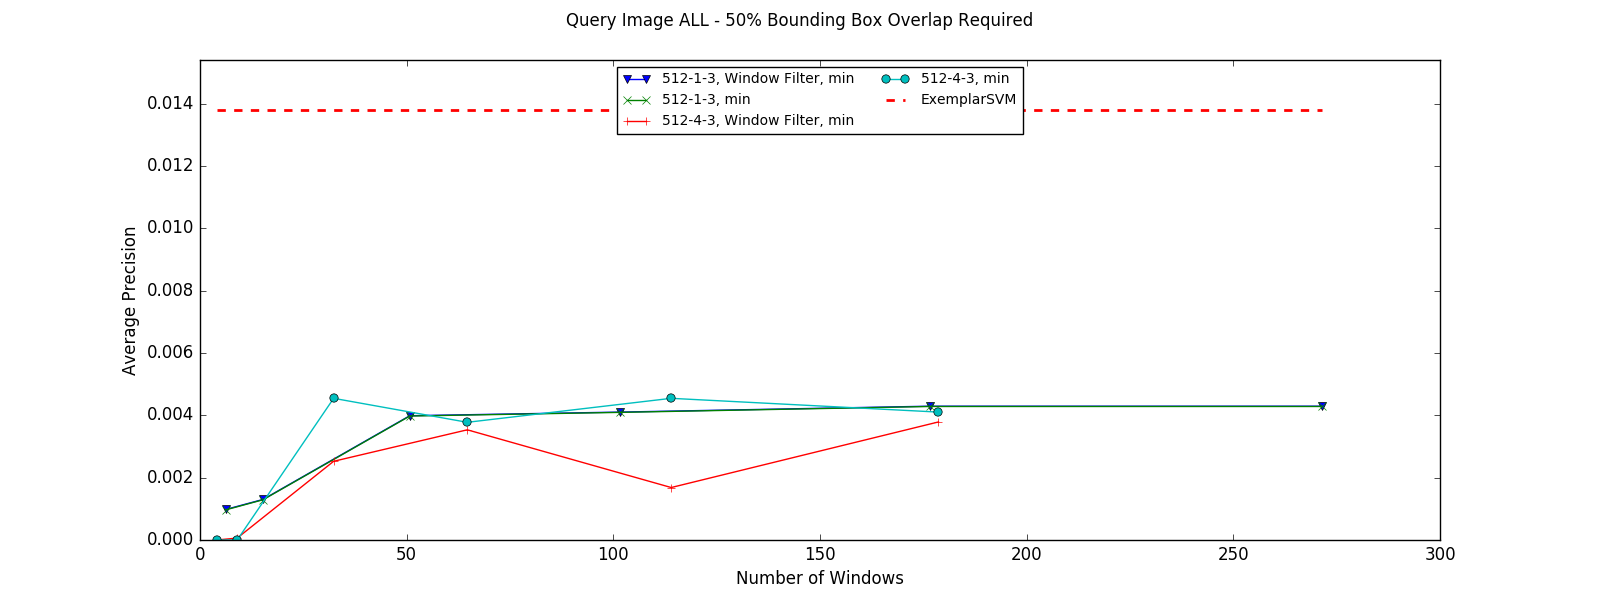
\includegraphics[width=\linewidth]{images/val_window_comparison-ALL}
\caption{Averaged detection performance of different windows compared to ExemplarSVM (2500 images)}
\label{fig:val_window_comparison-ALL}
\end{figure}


\begin{figure}
\centering
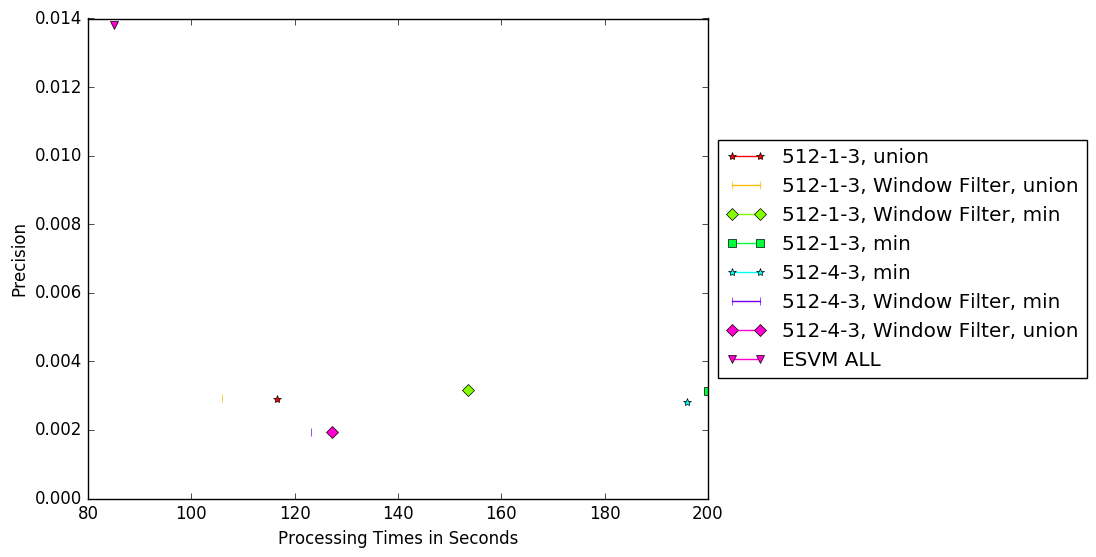
\includegraphics[width=0.7\linewidth]{images/val_t_vs_p-ALL}
\caption{Performance versus search time (2500 images)}
\label{fig:val_t_vs_p-ALL}
\end{figure}
